\section{EXTRA: Systems and Signals}
\subsection{Background}
\subsubsection{Complex Numbers}
Electrical engineers use the notation $j$ instead of $i$ for complex numbers.

\begin{equation}
    j^2 = -1 \quad \text{and} \quad \sqrt{-1} = \pm j
\end{equation}

Since $e^{j \theta} = \cos \theta + j \cos \theta$, we can have a polar representation of complex numbers as $z = re^{j \theta}$.
We also have the following facts that allow us to move between the forms and express in both polar and rectangular forms.
\begin{itemize}
    \item $a = r \cos \theta \quad b = r \sin \theta$
    \item $r = \sqrt{a^2 + b^2} \quad \theta = \tan^{-1} (\frac{b}{a}) $
\end{itemize} 

We can also represent the magnitude of $|z|$ as the radius $r$ which is the distance of the point $z$ from the origin.
The angle $\theta$ can similarly be represented as $\angle z$.

The conjugate $z^*$ of a complex number $z=a+jb$is defined as 
\begin{equation}
    z^8 = a - jb = re^{-j \theta},
\end{equation}
which is a mirror image of $z$ about the horizontal (real) axis.
We can easily see that the sum of a complex number and its conjugate is a real number equal to twice the real part of the number:
\begin{equation}
    z + z^* = (a+jb) + (a-jb) = 2a,
\end{equation}
and the difference of a complex number and its conjugate is an imaginary number equal to twice the imaginary part of the complex number:
\begin{equation}
    z - z^* = (a+jb) - (a-jb) = 2jb.
\end{equation}

The product of the two is the square of the magnitude
\begin{equation}
    zz^* = (a+bj)(a-bj) = a^2 -(jb)^2 = a^2 + b^2 = |z|^2.
\end{equation}

In simpler terms, $re^{j\theta}$ represents a point $z$ that has a distance $r$ from the origin and an angle $\theta$ with the horizontal axis.

When adding or subtracting complex numbers, the cartesian form is preferred due to its simplicity.
Conversely, for multiplying, dividing, or raising to a power, the polar form simplifies greatly compared to the cartesian form.

\subsubsection{Sinusoids}
For a sinusoid $x(t) = C \cos (2\pi f_0 t + \theta)$, we know that the sinusoid repeats itself every $2\pi n$ where $n \in \mathbb{Z}$.
The section $f_0 t$ is an integer whenever $t$ changes by $1/f_0$.
Commonly, $f_0$ is known as the frequency and $T_0 = \frac{1}{f_0}$ is known as the period.
$C$ is the amplitude and $\theta$ is the phase.

The variable $w_0$ is used frequently (radian frequency) to express $2\pi f_0$.
$w_0$ has units in radians whereas $f_0$ has units in hertz.
This leads to the following sinusoid representation
\begin{equation}
    x(t) = C \cos (w_0 t + \theta)
\end{equation}
where the the period $T_0 = \frac{2 \pi}{w_0}$.

\begin{figure}[htbp]
  \centerline{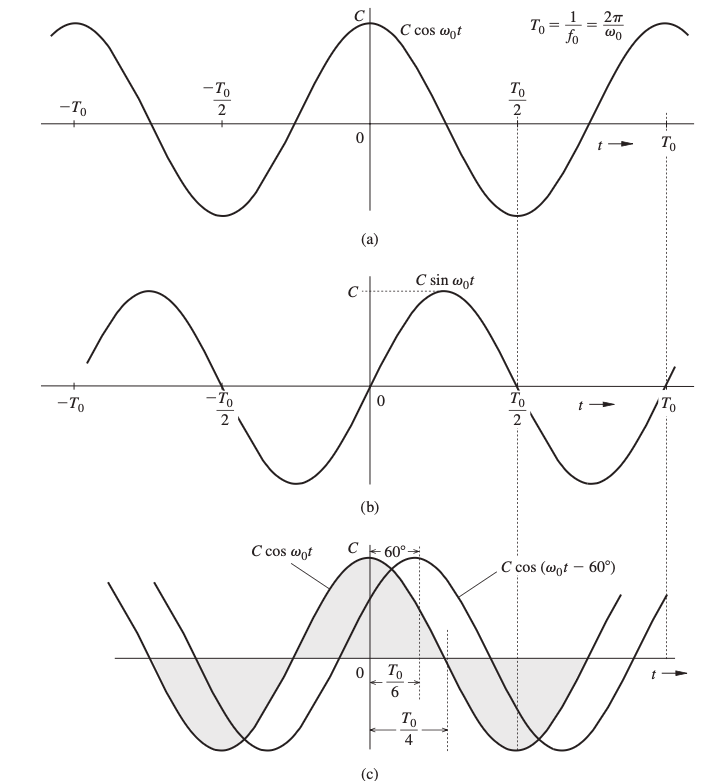
\includegraphics[width=0.75\textwidth]{../../images/example_sinusoids.png}}
  \caption{Some examples of different sinusoids}
  \label{fig:example_sinusoids}
\end{figure}

It is important to remember that getting from $\sin$ to $\cos$ is as simple as shifting by $\pi/2$
\begin{equation}
    C \cos(w_0 t - \pi/2) = C \sin w_0 t
\end{equation}

$\sin w_o t$ lags $\cos w_0 t$ by $\pi/2$.

We can add two sinusoids that have the same frequency easily.

\begin{equation}
    C \cos \theta \cos w_0 t - C \sin \theta \sin w_0 t = C \cos (w_0 t + \theta) = a \cos w_0 t + b \sin w_0 t 
\end{equation}

\subsubsection{Exponentially-Decaying Sinusoids}
An exponentially-decaying sinusoid has the form 
\begin{equation}
    Ae^{-at} \cos (\omega_0 t + \theta)
\end{equation}
\begin{figure}[htbp]
  \centerline{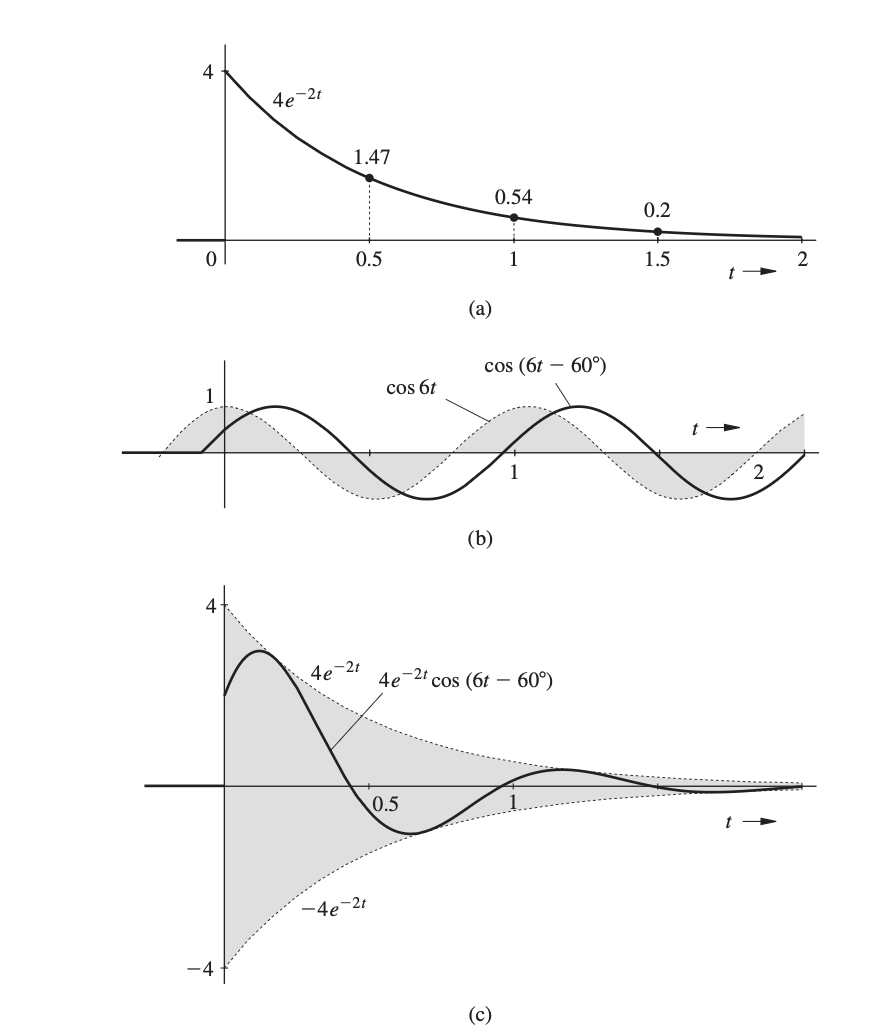
\includegraphics[width=0.75\textwidth]{../../images/drawing_exponential_sinusoids.png}}
  \caption{An example of combining an exponential and sinusoid into an exponentially-decaying sinusoid.}
  \label{fig:drawing_exponential_sinusoids}
\end{figure}

\subsubsection{Cramer's Rule}
A linear equation with the same amount of equations and unknowns $n$ can be solved with Cramer's Rule.
\begin{equation}
    x_k = \frac{|\textbf{D}_k|}{|\textbf{A}|} \quad k = 1,2,\dots, n
\end{equation}
This only occurs if the determinant of \textbf{A} is not zero and is therefore non-singular.

\subsubsection{Partial Fraction Expansion}
If we have a function that is a fraction of two polynomials, this function $F$ is improper if $m$ (the degree of the numerator polynomial) is larger than $n$ (the degree of the denominator).
It is proper if the converse holds.
\begin{equation}
    F(x) = \frac{P(x)}{Q(x)} = \frac{b_m x^m + b_{m-1} x^{m-1} + \dots + b_1 x + b_0}{a_n x^n + a_{n-1} x^{n-1} + \dots + a_1 x + a_0}
\end{equation}
An improper fraction can always be turned into the sum of a polynomial and a proper fraction ($m < n$).
There are a few ways that we can turn a rational function $F(x)$ into partial fractions.
Clearing fractions can be used by splitting into each partial fraction with their root denominators and then multiplying to remove fractions, and finally solving a system of equations.
The method of residues involves getting to a set of factors that are distinct for $Q(x)$ and then plugging them into the original $F(x)$ while excluding that root from the equation.
